\documentclass[12pt,reqno]{amsart}
\usepackage{./header, amssymb}

\hdr{Mathematical Statistics}{Chapter 12: Probabilistic graphical models}

\begin{document}

\bigskip

\prob Suppose that we have three binary random variables $X$, $W$, and $H$, which indicate whether a person exercises regularly ($X$), whether they are overweight ($W$), and whether they have heart disease ($H$). Discuss several causal structure involving these variables.













\vfill
\prob Let $X$ and $Y$ be binary random variables that indicate whether a person has \textit{hydromechanical trepidation syndrome} ($X$) and whether they test positive ($Y$) for it. Suppose that
	\[p(y=1 |x=1) = 0.98 \quad \text{and} \quad p(y=1 | x=0) = 0.1.
	\]
Express the flow of information from $X$ to $Y$ as a stochastic link by explicitly writing down a link function.


	






\vfill
\newpage
\prob Explicitly draw the full graphical structure for a plated linear regression model

\bigskip
\begin{center}
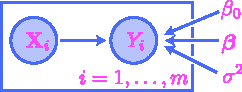
\includegraphics[scale=1.5]{lin-reg-00-plated.pdf}
\end{center}
\bigskip

when $m=3$.














\vfill
\prob Given a linear regression model with predictors $\mathbf{X}$, response $Y$, and parameters $\beta_0$, $\boldsymbol{\beta}$, and $\sigma^2$, we saw in class that
	\[ R \mid \mathbf{X} = \mathbf{x} \sim N(0, \sigma^2)
	\]
where $R = Y - \beta_0 - \mathbf{X}^\intercal \boldsymbol{\beta}$ is the error term. Prove this claim.











\vfill
\prob Compute the inverse of the sigmoid function $\sigma(x) = 1/(1+e^{-x})$. Interpret its meaning.













\vfill
\newpage
\prob The \textit{confusion matrix} for the logistic regression model discussed in class is given by
	\[\begin{array}{c|cc}
	& \hat{y}=0 & \hat{y} = 1 \\ \hline
	y=0 & 422 & 90 \\
	y=1 & 95 & 417
	\end{array}
	\]
where $y$ is the true class and $\hat{y}$ the predicted class of an instance in the dataset. In this problem, a \textit{positive} class label corresponds to $1$, while a \textit{negative} class label corresponds to $0$.

\medskip
\begin{enumerate}
\item Compute the \textit{accuracy} of the classifier, which is the proportion of correctly classified instances out of all total instances.\vfill
\item Compute the \textit{precision} of the classifier, which is the proportion of all true positive predictions out of all positive predictions. (High precision $=$ avoids false positives.)\vfill
\item Compute the \textit{recall} (or \textit{sensitivity}) of the classifier, which is the proportion of all true positive predictions out of all actual positive instances. (High sensitivity $=$ avoids false negatives.)\vfill
\item Discuss situations in which the primary interest is in classifiers with high precision, versus a situation in which the primary interest is high sensitivity.
\end{enumerate}







\vfill
\prob Describe a possible neural network architecture for datasets of the form
	\[(\mathbf{x}_1,y_1),(\mathbf{x}_2,y_2),\ldots,(\mathbf{x}_m,y_m) \in \mathbb{R}^n \times \mathbb{R},
	\]
where the $y_i$'s are drawn from a continuous random variable $Y$.

\vfill











\end{document}